\chapter{Een nieuwe UniProtKB-index voor Unipept}\label{ch:een-nieuwe-uniprotkb-index-voor-unipept}
In de vorige hoofdstukken hebben we suffixbomen, suffix arrays, FM-indices en R-indices verkend als indexstructuren die toegepast kunnen worden om een proteïnedatabank te indexeren.
Hieruit bleek dat een suffix array de laagste geheugenvereisten heeft tijdens het opbouwen.
In dit hoofdstuk gaan we dieper in op het opbouwen van een index voor UniProtKB gebruikmakende van een suffix array, en het in productie brengen ervan.
Aangezien we de huidige Unipept index willen vervangen door deze nieuwe indexstructuur behandelen we bovendien ook nog enkele extra gewenste features.

\section{Opbouwen van de SA}\label{sec:opbouwen-van-de-sa}
Zoals vermeld in sectie~\ref{subsec:opbouwen} levert een ruwe extrapolatie op dat we 1.2 TB RAM nodig hebben om een suffix array op te bouwen voor UniProtKB\@.
Hierbij wordt er echter van uitgegaan dat UniProtKB 500 keer meer proteïnen dan Swiss-Prot bevat.
Dit is een overschatting van de realiteit waar UniProtKB op dit moment \textit{slechts} $\pm$ 440 keer groter is.
Dit zorgt ervoor dat het opbouwen mogelijks al \textbf{haalbaar is op de HPC van UGent} waar nodes beschikbaar zijn tot 940 GB RAM\@.
Na dit te proberen bleek \textit{slechts} 740 GB RAM nodig.
Dit is minder dan verwacht omdat onder andere de NCBI taxonomy in het geheugen gehouden wordt.
Deze blijft even groot, onafhankelijk van de grootte van de proteïnendatabank.
Figuur~\ref{fig:build_uniprot} toont de nodige tijd en hoeveelheid geheugen om dit te realiseren.
\textbf{Opvallend hierbij is dat de libsais implementatie hier trager is dan libdivsufsort}, terwijl dit voor alle kleinere datasets net omgekeerd was.
Afhankelijk van de dataset is het ene algoritme dus sneller dan het andere.
Het geheugengebruik van beide algoritmen blijft echter erg gelijkaardig, wat het belangrijkste is voor ons.
\\
\begin{figure}[H]
    \centering
    \subfloat[Tijd nodig om een SA-index voor UniProtKB te bouwen.]{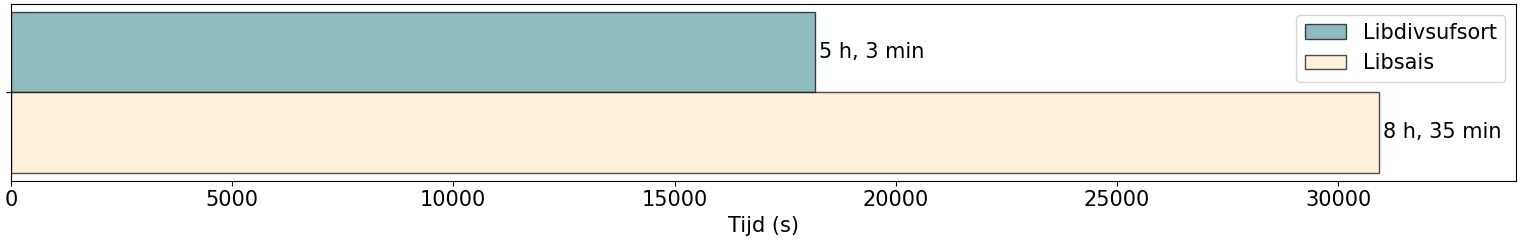
\includegraphics[width=\linewidth]{build_uniprot_time}}\\[4ex] % [4ex] om wat extra vertical spacing in te voegen

    \subfloat[Maximale hoeveelheid geheugen gebruikt tijdens het opbouwen van een SA-index voor UniProtKB.]{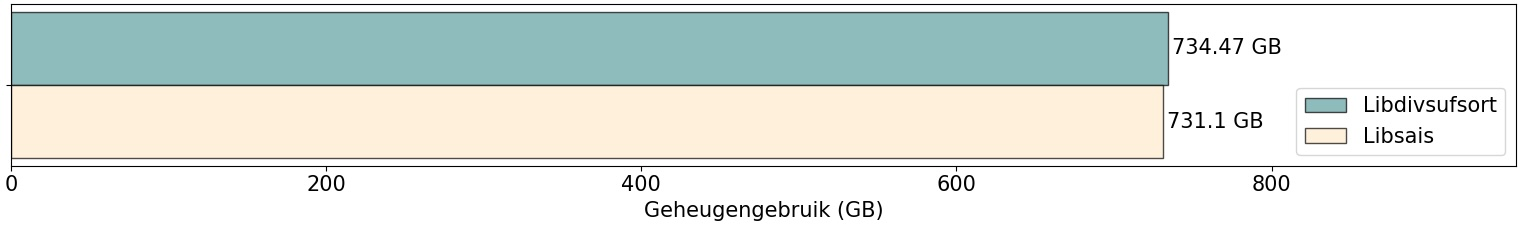
\includegraphics[width=\linewidth]{build_uniprot_memory}}
    \caption{Statistieken voor het opbouwen van een SA voor UniProtKB.}\label{fig:build_uniprot}
\end{figure}

\section{Een sparseness factor kiezen}
Een volgende stap na het opbouwen van de volledige SA bestaat uit het kiezen van de optimale sparseness factor.
Zoals eerder aangegeven in de conclusie van sectie~\ref{subsec:zoeken-in-sparse-suffix-arrays} willen we deze sparseness factor zo laag mogelijk houden, met als restrictie dat de sparse suffix array (SSA) nog steeds in het werkgeheugen moet passen.
Uit Figuur~\ref{fig:search_sparseness} (a) bleek namelijk dat het kiezen van een hogere sparseness factor een dramatische impact op de zoektijd van korte peptiden heeft.
Dit effect zal nog versterkt worden bij het gebruik van een grotere databank.
\\ \\
De beschikbare machines die Unipept hosten hebben elk $\pm$ 0.5 TB RAM ter beschikking.
Dit wil zeggen dat we de resulterende index hierin moeten krijgen, en ook nog genoeg ruimte moeten overlaten zodat de machine zeker niet crasht tijdens het hosten van de index en het verwerken van meerdere requests tegelijk.
Figuur~\ref{fig:uniprot_index_size_sparsenessfactors} toont een overzicht van de indexgrootte voor verschillende sparseness factors.
Aangezien we ongeveer 0.5 TB RAM ter beschikking hebben, zal \textbf{sparseness factor k = 3} de kleinste factor zijn die comfortabel in het geheugen past.
We hebben hiervoor namelijk al 322 GB RAM nodig.
Hierbij moet natuurlijk nog wat overhead gerekend worden voor de mapping van suffix naar proteïne, en alle annotaties die bij een proteïne horen bij te houden.
Bovendien bevatten deze servers ook nog andere databanken om verdere aggregaties te berekenen.
Indien we sparseness factor 2 zouden gebruiken komt de totale indexgrootte uit op $\pm$ 440 GB\@.
Dit op zich zou nog net in de machine passen, maar laat niet genoeg ruimte voor de andere processen.

\begin{figure}[h!]
    \centering
    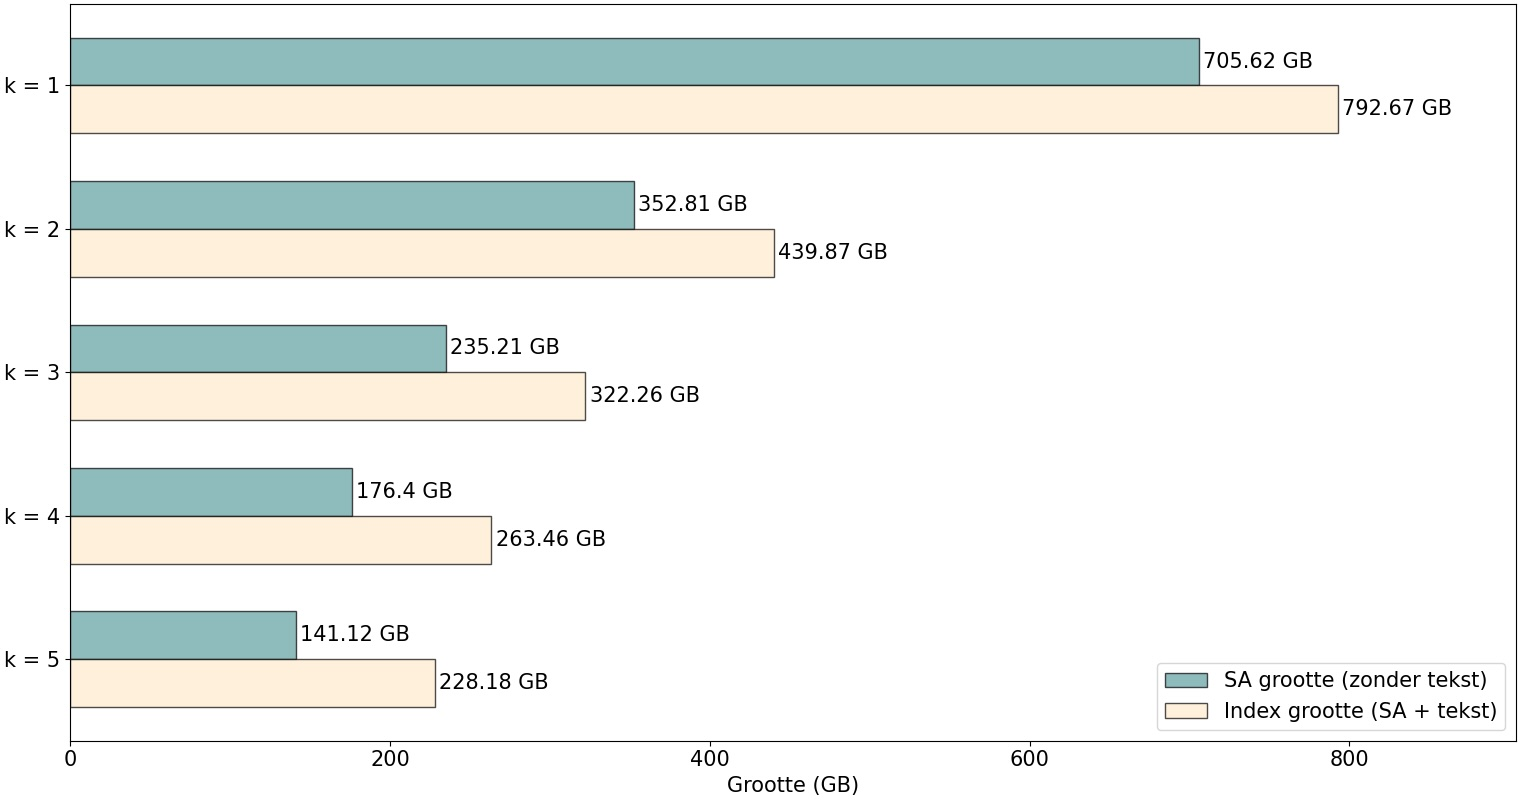
\includegraphics[width=0.8\linewidth]{uniprot_index_sizes}
    \caption{Grootte van de SA en totale index opgebouwd op UniProtKB voor sparseness factor $k = 1, 2, 3, 4, 5$.}
    \label{fig:uniprot_index_size_sparsenessfactors}
\end{figure}

\section{Isoleucine en leucine gelijkstellen}\label{sec:isoleucine-en-leucine-equivalentie}
Naast het vinden van exacte matches is het vinden van inexacte matches ook interessant.
Vooral het vinden van matches waarbij we de aminozuren I (isoleucine) en L (leucine) aan elkaar gelijkstellen is een belangrijke optie in de huidige Unipept index.
\textbf{Deze twee aminozuren kunnen niet gedifferentieerd worden door een massaspectrometer omdat ze een identieke massa hebben}.
Door deze restrictie is het voor onderzoekers erg nuttig om alle matches te vinden waar een I ook een L kan zijn, of omgekeerd.
Om deze vorm van inexacte matching toe te voegen aan de index gebruikmakende van een suffix array zijn er meerdere opties:
\begin{enumerate}
    \item \textbf{Twee indices:} Bouw een extra index waarbij in de tekst elke L ook door een I vervangen wordt, of vice versa.
    Bij het verwerken van een zoekopdracht wordt deze afgehandeld door de juiste index afhankelijk van de gekozen configuratie.
    Indien I en L gelijkgesteld worden hoeft er slechts één bijkomende operatie uitgevoerd te worden.
    Dit is dezelfde vervangoperatie die uitgevoerd is op de originele tekst bij het opstellen van de index.
    Deze optie wordt niet verder uitgewerkt omdat we willen vermijden dat we twee volledig aparte indices moeten hosten, waardoor het geheugengebruik zou verdubbelen.
    \item \textbf{Index waarbij I $\neq$ L:} Genereer de varianten van de gezochte peptide \textit{on the fly} tijdens het zoekproces.
    Hierbij kan gebruikgemaakt worden van het feit dat twee peptiden die identiek zijn, behalve dat elke locatie waar een I een L kan staan (of vice versa), een gelijkaardig zoekpad afleggen in de SA\@.
    Deze zoekpaden splitsen enkel wanneer het teken dat verwerkt wordt (uit de proteïnedatabank) tijdens de binary search een I, J, K of L is.
    Dit zorgt ervoor dat voor een willekeurig patroon een groot stuk van de zoekboom gemeenschappelijk zal zijn.
    Ook al zal dit ervoor zorgen dat we tijdens het zoekproces meestal snel kunnen snoeien, we zullen steeds $2^{q}$ opties moeten verkennen.
    Hierbij is $q$ de som van het aantal I's en L'en is in de peptide.
    \item \textbf{Index waarbij I = L:} Bouw de index voor een variant van de UniProtKB database.
    Hierbij vervangen we elke I door een L, of vice versa, en bouwen we dus een index op waarbij I gelijkgesteld is aan L\@.
    Tijdens het zoeken van een peptide doen we dezelfde vervanging, waarna we alle matches hebben waarbij I gelijkgesteld is aan L\@.
    Indien we I niet gelijk willen stellen aan L, kunnen we achteraf de foute matches wegfilteren aan de hand van de originele proteïnedatabank.
\end{enumerate}

In de volgende secties worden de tweede en derde aanpak verder uitgewerkt.

\subsection{Index waarbij I $\neq$ L}\label{subsec:index-waarbij-i-neq-l}
Wanneer de indexstructuur zelf gebouwd is met I niet gelijkgesteld aan L, moeten we alle verschillende IL-combinaties tijdens het zoekproces verkennen.
Hierbij is het echter belangrijk om te weten dat er ook bepaalde extreem slechte gevallen bestaan waarbij de zoekruimte erg groot wordt, en we niet efficiënt kunnen snoeien.
De sequenties waarop we zoeken zijn namelijk niet random verdeeld over alle karakters van het alfabet.
Biologisch gezien komen bepaalde aminozuursequenties veel vaker voor.
Eén van deze patronen zijn de zogenaamde \textit{leucine rich repeats}~\cite{leucine_rich_repeats}.
Dit zijn sequenties waarin een reeks L'en na elkaar voorkomt.
In UniProtKB bestaat er een \textbf{sequentie waar maar liefst 2397 L'en na elkaar voorkomen}.
Dit is de proteïne met \textit{accession number} \texttt{A0A1Q9EZQ0}.
Wanneer we nu ook weten dat in UniProtKB ook reeksen aan I's voorkomen zorgt dit voor bepaalde extreem slechte gevallen.
Zo is hier \textbf{ook een proteïne met 641 opeenvolgende I's} (accession number: \texttt{A0A5J4P3H7}).
In het slechtste geval zou een gebruiker dus een sequentie van 641 I's of L'en kunnen proberen te matchen.
Dit zorgt ervoor dat we in de zoekboom $2^{641} \approx 9.12 \cdot 10^{192}$ opties moeten proberen.
Het grootste deel van deze opties zal niet voorkomen, waardoor de takken van deze boom allemaal extreem kort zullen zijn.
Dit zal echter verwaarloosbaar zijn ten opzichte van het gigantisch aantal opties.
Om dit in perspectief te plaatsen: Men schat dat er in het totaal $10^{79}$ atomen in het universum zijn~\cite{atoms_in_universe} en dat het universum ongeveer $4.36^{20} \approx 6.16 \cdot 10^{12}$ milliseconden oud is~\cite{age_universe}.
Zelfs als het controleren van één optie minder dan een milliseconde duurt, dan zou dit dus nog onmogelijk zijn.
\textbf{Om de zoektijd en het geheugengebruik te beperken, hebben we ervoor gekozen om twee vormen van restricties op te leggen wanneer I en L gelijkgesteld worden}.
\begin{enumerate}
    \item Laat maximaal 5 seconden aan zoektijd per peptide toe.
    \item Laat per peptide in totaal maximaal 34 I's en L'en toe.
\end{enumerate}
Deze twee restricties samen moeten de servers deels helpen beschermen tegen Denial of Service attacks.
In de praktijk wordt normaal de tijdslimiet van 5 seconden eerst bereikt.
Dit vertaalt zich naar een sequentie van ongeveer 25 I's of L'en.
Elke keer we één extra teken zouden willen toelaten verdubbelt de zoektijd.
Zo duurt het al één minuut om een sequentie met 30 opeenvolgende I's of L'en te zoeken.
Wanneer we echter nog veel meer I's of L'en toelaten stuiten we vrij snel op een geheugenlimiet.
Om te voorkomen dat het programma meer geheugen probeert te vragen dan dat de server heeft, waarna het crasht, hebben we beslist maximaal 34 I's of L'en toe te laten.
In het slechtste geval gebruikt één enkele thread hierbij iets meer dan 2 GB RAM\@.
Aangezien het zoeken multithreaded is, moeten we dus zeker 20 GB aan vrij geheugen voorzien wanneer de index ingeladen is.
\textbf{Wanneer we deze limieten testen door alle testpeptidebestanden te zoeken in de volledige UniProtKB databank worden deze limieten geen enkele keer bereikt}.
\\ \\
In de praktijk vertaalt het gelijkstellen van I en L op deze manier zich naar een \textbf{vrij kleine overhead}.
Deze beperkte overhead valt te zien in Figuur~\ref{fig:uniprot_search}.
Deze figuur toont ook onmiddellijk de zoekperformantie waarbij I $\neq$ L op UniProtKB\@.
Zoals verwacht op basis van de resultaten voor de kleinere Swiss-Prot en Human-Prot proteïnedatabanken, is dit zoeken inderdaad extreem snel.
% TODO: schrijf hier iets bij in vergelijking met de huidige unipept index qua snelheid

\begin{figure}[ht]
    \centering
    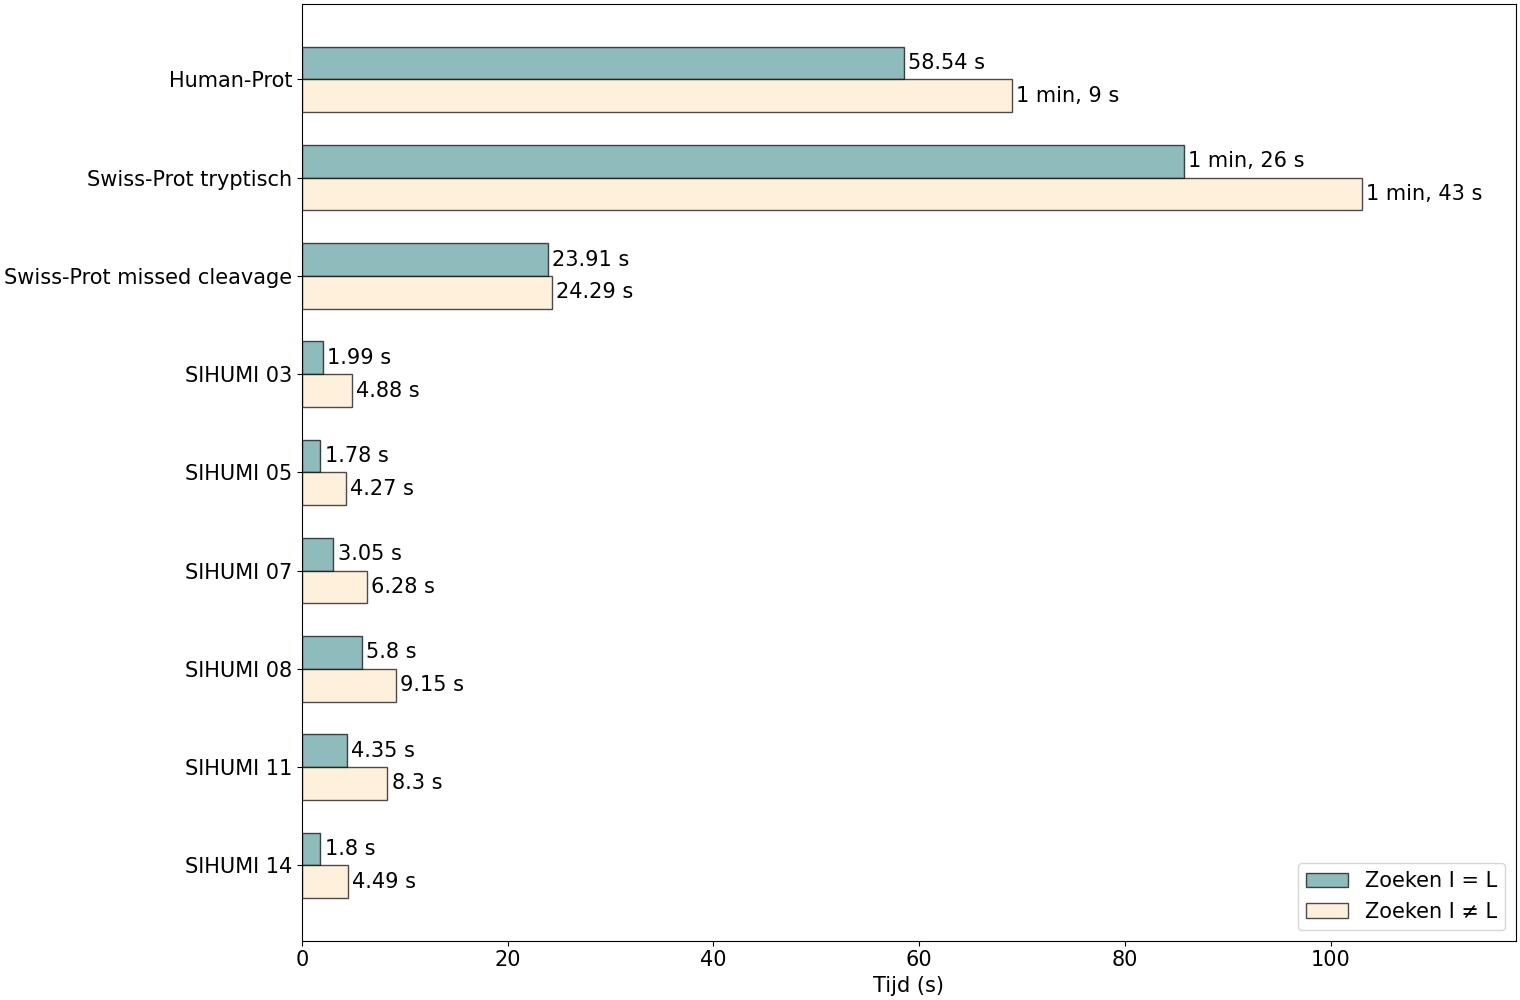
\includegraphics[width=0.95\linewidth]{uniprot_searchtime_standard_vs_il_equality}
    \caption{Zoektijd in UniProtKB (Swiss-Prot + TrEMBL) met en zonder het gelijkstellen van I en L met een SA met sparseness factor $k = 3$. De index zelf is opgebouwd op basis van een tekst waar I $\neq$ L.}
    \label{fig:uniprot_search}
\end{figure}

\subsection{Index waarbij I = L}
Een andere optie om zoeken waarbij I en L gelijkgesteld zijn mogelijk te maken is door de index specifiek voor dit geval op te bouwen.
Hierbij wordt in de originele tekst elke L vervangen door een I, of vice versa, om op deze aangepaste tekst een index te bouwen.
Wanneer we in de gezochte peptiden hetzelfde doen, vinden we alle matches, waarbij een I en L gelijkgesteld zijn.
Dit is duidelijk erg simpel, en bovendien efficiënt.
\\ \\
Door het zoekproces licht aan te passen, kunnen we bovendien nog steeds de matches vinden waarbij I $\neq$ L\@.
Dit kan via volgend stappenplan:
\begin{enumerate}
    \item \textbf{Zoek alle matches} in de SA, waarbij I = L\@.
    Hiervoor moeten we in elke peptide dezelfde vervangoperatie uitvoeren als tijdens het bouwen van de suffix array.
    \item \textbf{Filter de ongeldige matches weg}.
    Dit kunnen we doen door voor alle matches te controleren op elke positie waar een I of L is, als daar hetzelfde teken staat als in de tekst.
    Wanneer in de peptide een L staat, en de tekst een I (of omgekeerd), wil dit zeggen dat deze match ongeldig is, want ze is enkel gevonden vanwege het gelijkstellen van I aan L tijdens het zoeken.
    Merk op dat we hiervoor de originele tekst nodig hebben, en niet de aangepaste tekst die gebruikt is bij het bouwen van de suffix array.
    Gelukkig moeten we niet allebei deze teksten in het geheugen houden, via enkele kleine aanpassingen tijdens het zoeken kan de originele tekst perfect gebruikt worden om te zoeken in de suffix array van de gemodificeerde tekst.
\end{enumerate}

Dit stappenplan is niet alleen \textbf{simpel}, maar het bevat ook \textbf{geen extreem slechte gevallen} zoals bij de index waarbij we I $\neq$ L stellen, en dan alle opties proberen verkennen.
Bovendien is ook de impact van de filterstap beperkt aangezien enkel locaties waar een I of L staat in de peptide gecontroleerd moeten worden.
Andere tekens moeten we nooit controleren, aangezien het zoeken in de SA ons al garandeert dat deze overeenkomen.
Er is dus geen nood aan een combinatie van systemen die de server moeten beschermen tegen de slechtste gevallen, die extreem lang konden duren, en bovendien ook veel geheugen vereisen.
\\ \\
Naast deze voordelen blijkt ook dat deze manier van zoeken iets sneller is in het algemeen.
Dit valt te zien in Figuur~\ref{fig:uniprot_search_il_equal}.
Een laatste voordeel is dat het gelijkstellen van I en L de standaard optie is in de huidige Unipept UI\@.
Dit is net ook wat hier het minste werk vereist tijdens het zoeken.
Vanwege al deze voordelen kiezen we ervoor om van deze zoekstrategie gebruik te maken.

\begin{figure}[ht]
    \centering
    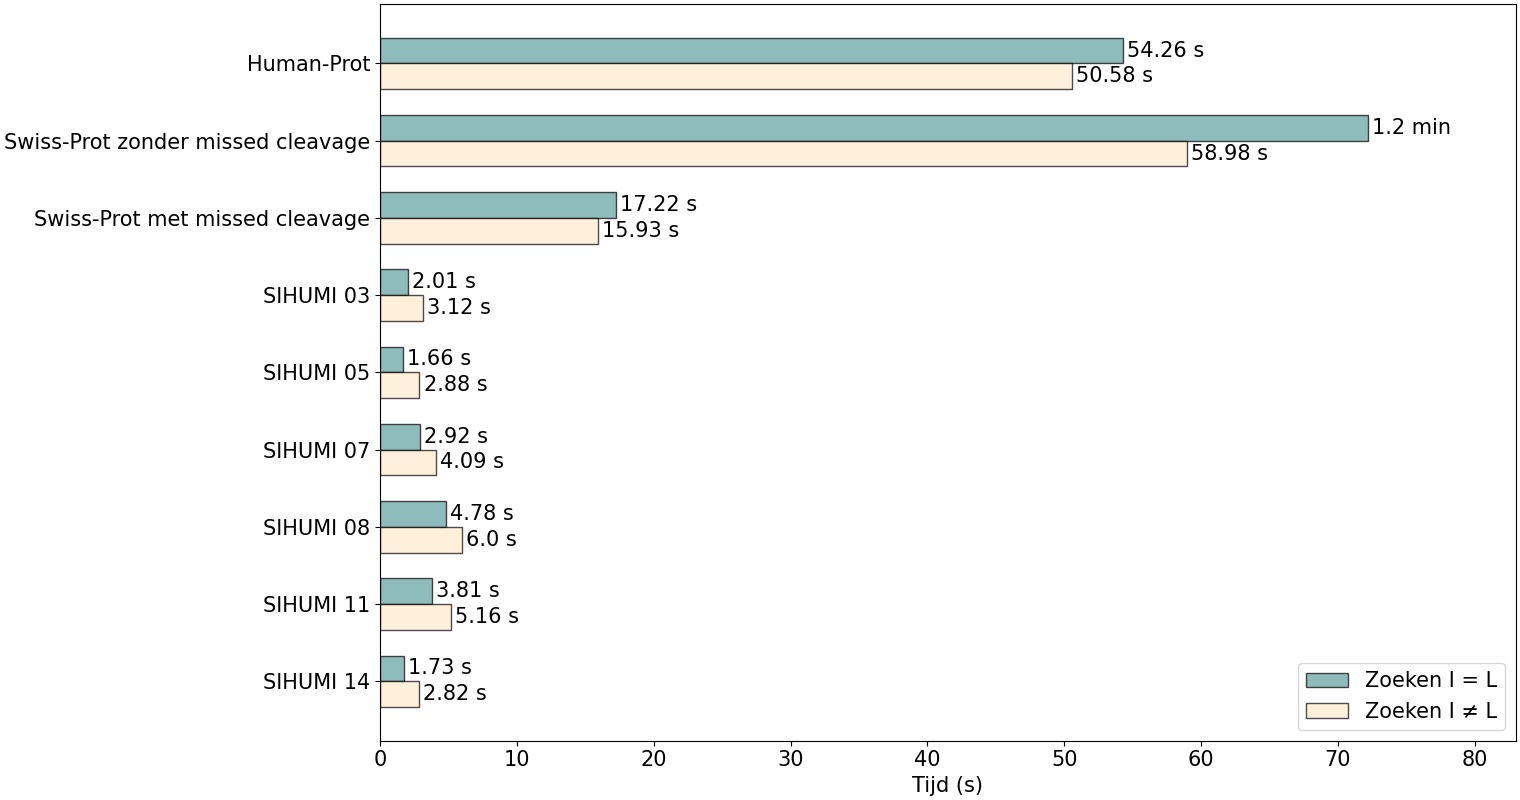
\includegraphics[width=0.95\linewidth]{uniprot_searchtime_standard_vs_il_equality_il_equal_index}
    \caption{Zoektijd in UniProtKB (Swiss-Prot + TrEMBL) met en zonder het gelijkstellen van I en L met een SA met sparseness factor $k = 3$. De index zelf is opgebouwd op basis van een tekst waar I = L.}
    \label{fig:uniprot_search_il_equal}
\end{figure}

Eén iets merkwaardig is dat voor onze kleinere SIHUMI testbestanden het zoeken met I $\neq$ L sneller is, ook al is dit net minder werk.
Dit komt omdat zonder dit filteren er meer resultaten zijn.
Deze extra resultaten moeten allemaal meegenomen worden in het berekenen van de LCA*, maar ook tijdens het serializeren van de resultaten naar een JSON-bestand.
Bovendien zorgt een grotere hoeveelheid data ook voor een tragere doorstroming van de index naar de Unipept API\@.
Bij de grotere testbestanden wordt er in verhouding meer tijd aan het zoeken gespendeerd, waardoor daar de verwachte tijdwinst wel zichtbaar is.

\section{Taxonomische analyse}\label{sec:taxonomische-analyse}
Door het gebruik van suffix arrays moet de taxonomische analyse volledig uitgevoerd worden tijdens het zoekproces zelf.
Dit heeft zowel voor- als nadelen.
\\ \\
Het grootste nadeel is de \textbf{extra overhead per zoekopdracht}.
In de oude index was het enkel nodig alle matches te zoeken, waarna de voorberekende LCA onmiddellijk opgehaald kon worden.
Nu moeten we deze LCA ook nog berekenen.
Indien we dit zouden willen oplossen is er nood aan een manier om de boomstructuur te reconstrueren op een geheugenefficiënte manier.
Hiervoor zijn de extra tabellen van Enhanced Suffix Arrays nodig.
\\ \\
Anderzijds zijn er ook enkele voordelen verbonden met het berekenen tijdens het zoekproces zelf.
Zo hebben we \textbf{minder geheugen} nodig, wat erg belangrijk is aangezien het geheugengebruik al erg hoog is tijdens het opbouwen van de suffix array.
Bovendien laat dit ook toe dat we vrij kunnen kiezen welke aggregatiemethode we gebruiken.
De oude Unipept index maakte gebruik van een (minder interessante) variant van \textbf{LCA*}.
Dit werd gedaan om het voorberekenen efficiënter te maken.
Bij suffixbomen hebben we zelf gebruik moeten maken van de standaard LCA methode om dit op te lossen.
Bij suffix arrays kunnen we vrij gebruik maken van LCA*, en blijft de performantie bovendien erg goed.
Een laatste, belangrijk, voordeel is dat er \textbf{geen extra werk nodig is om de taxon IDs van alle matches op te halen}.
In de huidige Unipept index is hier een significante hoeveelheid extra werk voor nodig, wat resulteert in een bottleneck bij de Peptonizer2000 tool~\cite{pep_gm}.


\section{Functionele analyse}\label{sec:functionele-analyse}
Een laatste feature die de nieuwe index moet ondersteunen is de functionele analyse uit Unipept.
Deze analyse wordt uitgevoerd door de verschillende GO, EC en INTERPRO termen die horen bij de gevonden matches te tellen.
Elk van deze termen is een korte string van 5 à 10 karakters lang, en kan vrij eenvoudig mee ingelezen worden en per proteïne bijgehouden worden.
Al deze annotaties samen, maken het databankbestand dat ingelezen wordt om de index mee op te bouwen ongeveer 24 GB groter.
Wanneer we deze informatie allemaal ingeladen hadden, bleek het programma echter ongeveer 105 GB extra RAM te gebruiken.
De verklaring hiervoor is dat Rust 24 bytes overhead heeft per vector, en 24 bytes overhead per string.
Om deze annotaties bij te houden, hadden we net één vector per proteïne nodig, en die vector bevatte een reeks aan korte strings (de annotaties zelf).
Om dit op te lossen heeft Tibo Vande Moortele een simpele compressiebibliotheek\footnote{\url{https://github.com/unipept/unipept-index/tree/main/fa-compression}} ontwikkeld voor deze annotaties.
Hierbij worden 2 karakters uit een annotatie gecomprimeerd naar 1 byte, en kunnen bovendien enkele tekens weggelaten worden.
Na het gebruik van deze bibliotheek resulteert dit in \textbf{10.5 GB extra geheugengebruik}, wat in de context van de al 320 GB grote index (wanneer de tekst ook meegerekend wordt) bijna verwaarloosbaar is.
Aangezien ook deze analyse \textit{on the fly} uitgevoerd wordt, heeft ook dit een negatieve impact op de performantie.
De volgende sectie gaat dieper in op de performantie van de finale indexstructuur.

\section{Vergelijking met andere tools}\label{subsec:vergelijking-met-andere-tools}
Naast Unipept zijn er nog andere tools die UniProtKB doorzoeken.
In deze sectie vergelijken we de performantie en eigenschappen van Unipept met de \textbf{Uniprot Peptide search tool}, de \textbf{Expasy ScanProsite tool}.
We zullen de versie van Unipept die de nieuwe index gebruikt Unipept 6.x noemen, aangezien de nieuwe index gebruikt zal worden vanaf Unipept 6.0, terwijl de oude versie Unipept 5.x genoemd wordt.
Vanwege de beperkte performantie van een aantal van deze tools zullen we ons beperken tot het opzoeken van één willekeurige peptide \texttt{ISPAVLFVIVILAVLFFISGLLHLLVR}.
Als referentie gebruiken we de zoektijd Unipept 6.x waarbij, zoals eerder vermeld, sparseness factor $k = 3$ gebruikt wordt.
Hierbij duurt het zoeken van de peptide \textbf{$\pm$ 3 milliseconden} en levert deze 50 matches op.
Wanneer we I en L gelijkstellen duurt dit opnieuw ongeveer 3 milliseconden, maar levert dit wel 52 matches op.
Hierbij wordt natuurlijk geen extra tijd geïntroduceerd door een API call over het internet aangezien deze index (nog) niet publiek beschikbaar is.

\subsection{UniProt peptide search tool}
De UniProt peptide search tool~\cite{uniprot_search_paper, uniprot_search_site} is een onderdeel van de UniProt site en laat toe om alle voorkomens van een bepaalde peptide te vinden in de volledige UniProtKB databank.
Als opties kunnen we kiezen om enkel in Swiss-Prot te zoeken, of in Swiss-Prot en TrEMBL\@.
Voor beide databanken kunnen we kiezen of we I en L aan elkaar willen gelijkstellen.
Deze features komen exact overeen met de eigenschappen van onze nieuwe indexstructuur, met de uitzondering dan Unipept extra analyses aanbiedt.
Qua performantie is deze tool echter extreem onstabiel.
Zo duurt het zoeken van \texttt{ISPAVLFVIVILAVLFFISGLLHLLVR} in de volledige UniProtKB databank \textbf{enkele seconden tot zelfs 20 minuten}.
Bovendien vermoeden we ook dat er een vorm van caching toegepast wordt aangezien het zoeken voor een tweede keer zo goed als onmiddellijk het resultaat geeft.
Dit maakt het benchmarken extreem moeilijk.
Zoals verwacht zijn de gevonden matches identiek aan de matches die onze nieuwe indexstructuur vindt.
Naast de variabele performantie faalt deze tool ook regelmatig tijdens het zoeken en ophalen van de resultaten.
\\ \\
Vanwege de extreem gelijkaardige mogelijkheden van deze tool hebben we contact opgenomen met UniProt om de vergelijking meer compleet te maken.
Hun eigen index werkt op basis van Apache Lucene\footnote{\url{https://lucene.apache.org/}}, waarbij alle proteïnen opgesplitst worden in 3-grammen.
Volgende sectie bevat de gestelde vragen, met de gegeven antwoorden.

\begin{description}[style=nextline]
    \item[How much memory is needed to build the index structure?]
    Answer: There is no specific requirement for the RAM.
    One of our users had tested that it works with 32 GB RAM\@.
    \item[How long does it take to build the index?]
    Answer: It depends on the hardware.
    We usually run it in a machine with 256 GB RAM to index the UniProtKB sequences plus the related information.
    It can take 1 to 2 days depending on how busy the machine is.
    \item[How much memory is needed to host the index?]
    Answer: We had been running the PeptideSearch services in a server with 256 GB RAM for many years and upgraded the RAM to 512 GB to improve the performance.
    \item[How many requests do you handle per day?]
    Answer: There are around 350 searches per day in April.
    \item[How many peptides does the average request contain?]
    Answer: Around 80\% of the cases search one peptide.
    \item[What percentage of requests treat isoleucine and leucine as equivalent? ]
    Answer: Around 6\% of the cases treat isoleucine=leucine.
    \item[What is the average time needed to handle 1 request? During our own testing we noticed that the performance can vary a lot from request to request. Is there an explanation for this?]
    Answer: If you are using the tool on our website, response times can vary due to several reasons:
    \begin{enumerate}
        \item Load of the server running PeptideSearch (currently running at PIR in Delaware, US)
        \item Load/availability of the dispatching server which is located at the EBI, UK)
    \end{enumerate}
\end{description}

Uit deze antwoorden kunnen we concluderen dat hun index lagere geheugenvereisten heeft.
Vermoedelijk komt dit door Apache Lucene geen hard-limit heeft om de index te kunnen gebruiken.
Het zal echter zoveel geheugen proberen gebruiken als het toegewezen krijgt, om zo onder andere caching toe te passen.
Dit verklaart waarschijnlijk ook deels de variabele performantie.
Afhankelijk van eerdere zoekopdrachten zijn verschillende stukken van de index waarschijnlijk sneller doorzoekbaar.
\\ \\
Interessant is ook dat 80\% van de zoekopdrachten uit één peptide bestaan, en dat slechts in 6\% van de gevallen I en L gelijkgesteld worden.
Dit is net het tegenovergestelde van de geregistreerde requests bij Unipept.
Vermoedelijk komt het verschil bij het gelijkstellen van I en L doordat dit standaard aan staat bij Unipept, terwijl dit bij UniProt net standaard uit staat.

\subsection{Expasy ScanProsite tool}
De Expasy ScanProsite tool~\cite{scanprosite} laat toe om aan de hand van motieven die lijken op reguliere expressies allerlei patronen te zoeken.
De beschrijving van motieven laat toe om onder andere wildcards, karakterklassen\footnote{Hiermee bedoelen we het toelaten van een reeks aan tekens op een bepaalde plaats. Dit is gelijkaardig aan de \texttt{[ABC]} syntax uit reguliere expressies, waar we een A, B of C toelaten.}, inverse klassen en herhalingen te specificeren.
De flexibiliteit van dit systeem is dus een sterk voordeel.
Een nadeel van deze tool is dat niet de volledige UniProtKB databank doorzocht wordt.
Er wordt enkel rekening gehouden met proteïnen die deel uit maken van een \textit{reference proteome}\footnote{Deze zogenaamde \textit{reference proteomes} zijn een collectie van proteïnen die door een bepaald organisme gemaakt kunnen worden, en die bovendien taxonomisch belangrijk bevonden worden. Deze laatste voorwaarde wil dus zeggen dat dit niet zomaar van elk organisme is, enkel van een selecte groep organismes die op basis van verschillende factoren belangrijk bevonden wordt. Een voorbeeld hiervan is de \textit{human reference proteome}. Dit zijn alle proteïnen die door een mens aangemaakt kunnen worden.}.
Dit komt erop neer dat ze bij UniProt 2024\_01 \textbf{slechts rekening houden met 85\thinspace152\thinspace388 van de 249\thinspace751\thinspace891 proteïnen}.
Wanneer we de zoekperformantie testen, duurt het zoeken van de ene peptide zo'n \textbf{5.5 minuten} zonder gelijkstellen van I en L en 10 minuten met het gelijkstellen van I en L\@.
Hierbij zijn er slechts 30 resp. 32 matches gevonden, wegens de deelverzameling van proteïnen die gebruikt wordt.

\subsection{Unipept 5.x}
Unipept 5.x kan, \textbf{op voorwaarde dat je peptide tryptisch is}, alle matches te vinden in UniProtKB met de optie om I en L gelijk te stellen.
Onze willekeurig gekozen test peptide is tryptisch, dus vindt deze index zoals verwacht alle matches.
Bovendien gebeurt dit gebruikmakende van een API call in \textbf{$\pm$ 4 milliseconden}, wat duidelijk extreem veel sneller is dan de andere bestaande opties.
Opnieuw is de zoektijd hier al zo klein dat de invloed van het gelijkstellen van I en L niet te meten valt.
Het is echter een grote beperking dat dit enkel werkt voor tryptische peptiden, of peptiden met zogenaamde \textit{missed cleavages}.
Volgend voorbeeld illustreert dit.
Stel dat we nu de peptide \texttt{ILAKLFIS} zoeken.
Dit is geen tryptische peptide en bijgevolg kunnen er geen matches gevonden worden.
De nieuwe indexstructuur vindt echter 14 matches zonder I en L gelijk te stellen, en 207 matches bij het gelijkstellen van I en L\@.
\\ \\
Tot slot vergelijken we de zoektijd van Unipept 6.x en 5.x in meer detail aangezien één peptide hier geen goed zicht op geeft.
Hierbij berekenen beide indices ook de functionele en taxonomische analyses.
Het is belangrijk dat dit meegenomen worden tijdens het meten van de zoektijd, aangezien dit fundamentele functies van Unipept zijn.
We bekijken twee scenario's om zo een goed zicht op de performantie te krijgen.
In het eerste geval houden we rekening met \textit{missed cleavages}.
Dit is het meest realistische geval, aangezien stalen in de praktijk altijd \textit{missed cleavages} bevatten.
Figuur~\ref{fig:new_vs_old_unipept} geeft een overzicht voor de zoektijd op de SIHUMI peptidebestanden.
Hieruit blijkt dat Unipept 6.x 10 tot 100 keer sneller is dan Unipept 5.x.
Het andere geval is wanneer we een peptidebestand verwerken waarin enkel tryptische peptiden voorkomen.
Dit is niet realistisch, maar is het beste scenario voor Unipept 5.x aangezien de \textit{advanced missed cleavage handling} dan niet gebruikt moet worden.
Figuur~\ref{fig:new_vs_old_unipept_tryptic} toont het verschil in zoektijd tussen Unipept 6.x en 5.x voor het tryptische Swiss-Prot peptidebestand.
Ter herinnering: dit bestand bestaat uit 100\thinspace000 tryptische peptiden.
Hieruit blijkt dat Unipept 6.x 33\% trager is dan Unipept 5.x wanneer I $\neq$ L, maar is de performantie erg gelijkaardig wanneer I = L\@.
Dit verschil is erg acceptabel, vooral omdat we eigenlijk altijd rekening willen houden met \textit{missed cleavages}.
De enige reden dit amper gedaan werd in Unipept 5.x, is vanwege de grote impact op de performantie.
Bovendien kan Unipept 6.x ook ingezet worden voor niet-tryptische peptiden, wat niet mogelijk was voor Unipept 5.x en eerder.

\begin{figure}[h]
    \centering
    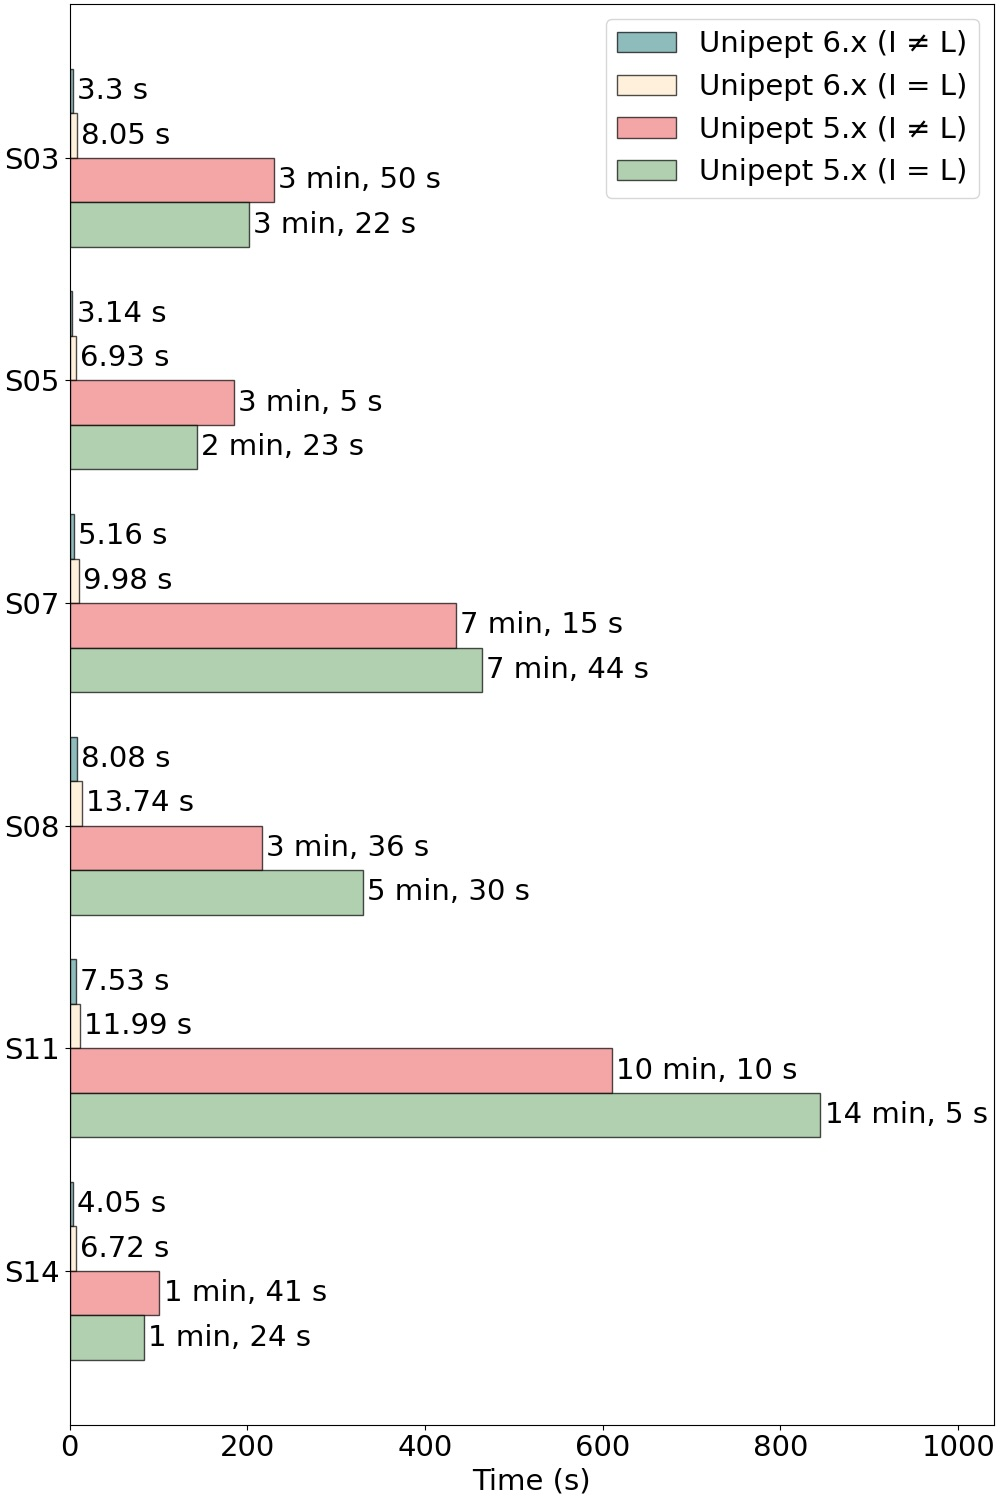
\includegraphics[width=0.85\linewidth]{new_vs_old_unipept}
    \caption{Unipept 6.x vs Unipept 5.x voor de SIHUMI peptidebestanden. Unipept 5.x is uitgevoerd met \textit{filter duplicate peptides} af, en \textit{advanced missed cleavage handling} aan. Op deze manier zullen beide versies alle peptiden zoeken, en ook \textit{missed cleavages} afhandelen. Merk op dat Unipept 6.x altijd \textit{missed cleavages} zal zoeken, en bovendien zelfs peptiden zal vinden die op een arbitraire manier gesplitst zijn.}
    \label{fig:new_vs_old_unipept}
\end{figure}

\begin{figure}[h]
    \centering
    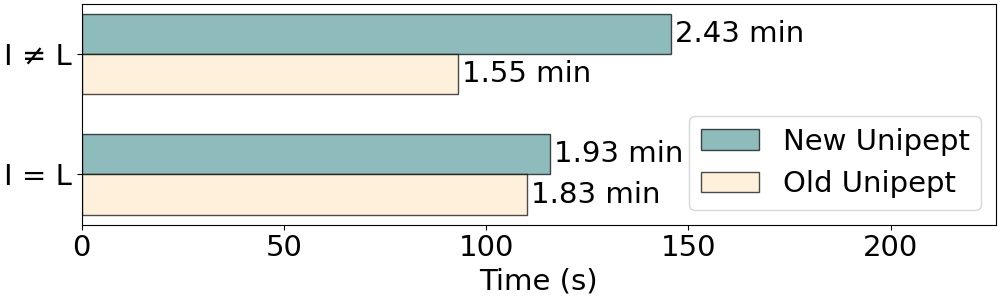
\includegraphics[width=0.85\linewidth]{new_vs_old_unipept_tryptic}
    \caption{Unipept 6.x vs Unipept 5.x voor het tryptische Swiss-Prot peptidebestand. Unipept 5.x is uitgevoerd met \textit{filter duplicate peptides} af, en \textit{advanced missed cleavage handling} af. Dit is het beste scenario voor Unipept 5.x, aangezien er geen \textit{missed cleavages} aanwezig zijn, en deze ook niet gezocht worden. Merk op dat Unipept 6.x wél \textit{missed cleavages} verwerkt, aangezien dit geen invloed heeft op de performantie bij de nieuwe indexstructuur.}
    \label{fig:new_vs_old_unipept_tryptic}
\end{figure}
\newpage
\section{Overzicht geheugenverbruik}
In de vorige secties zijn verschillende extra onderdelen besproken om de functionaliteiten van Unipept toe te voegen aan de nieuwe index.
Al deze extra onderdelen vragen extra geheugen, wat het totale geheugengebruik laat oplopen tot net geen 350 GB\@.
Figuur~\ref{fig:uniprot_memory_treemap} geeft een overzicht van het geheugenverbruik per onderdeel.
De volgende opsomming herhaalt kort voor elk onderdeel en welke rol deze speelt in het geheel.

\begin{itemize}
    \item Sparse suffix array: De sparse suffix array die opgebouwd werd op basis van de volledige UniProtKB databank.
    Op basis hiervan zoeken we efficiënt alle suffixen waarmee een peptide matcht.
    \item Tekst: Dit is de UniProtKB databank, waarbij alle proteïnen geconcateneerd worden tot één lange string.
    Tussen elke proteïne hangt hetzelfde, unieke scheidingsteken, en op het einde van de tekst een ander uniek teken.
    \item Functionele annotaties: De gecomprimeerde functionele annotaties die beschreven zijn in sectie~\ref{sec:functionele-analyse}.
    Op basis van deze annotaties wordt de functionele analyse van Unipept uitgevoerd.
    \item UniProt accession numbers: Elke proteïne in UniProtKB heeft een uniek ID (accession number).
    Voor elke proteïne die matcht met de gezochte peptide wordt dit ID als onderdeel van de output teruggegeven.
    \item Taxonomische annotaties: Het taxon ID dat per proteïne bijgehouden wordt.
    Op basis van deze taxon IDs wordt de LCA* van alle gevonden matches berekend.
    \item Suffix → proteïne: De sparse mapping die beschreven is in sectie~\ref{subsec:mapping-van-suffix-naar-proteine}.
    Deze mapping wordt gebruikt om de bijhorende proteïne te vinden van een gematchte suffix.
    \item NCBI taxonomy aggregator: Een object dat de gebruikte NCBI taxonomy om de LCA* aggregaties uit te voeren bevat.
    Aangezien deze opgebouwd wordt op basis van de NCBI taxonomy, is de grootte hiervan onafhankelijk van de gebruikte proteïnedatabank.
\end{itemize}

\begin{figure}[h]
    \centering
    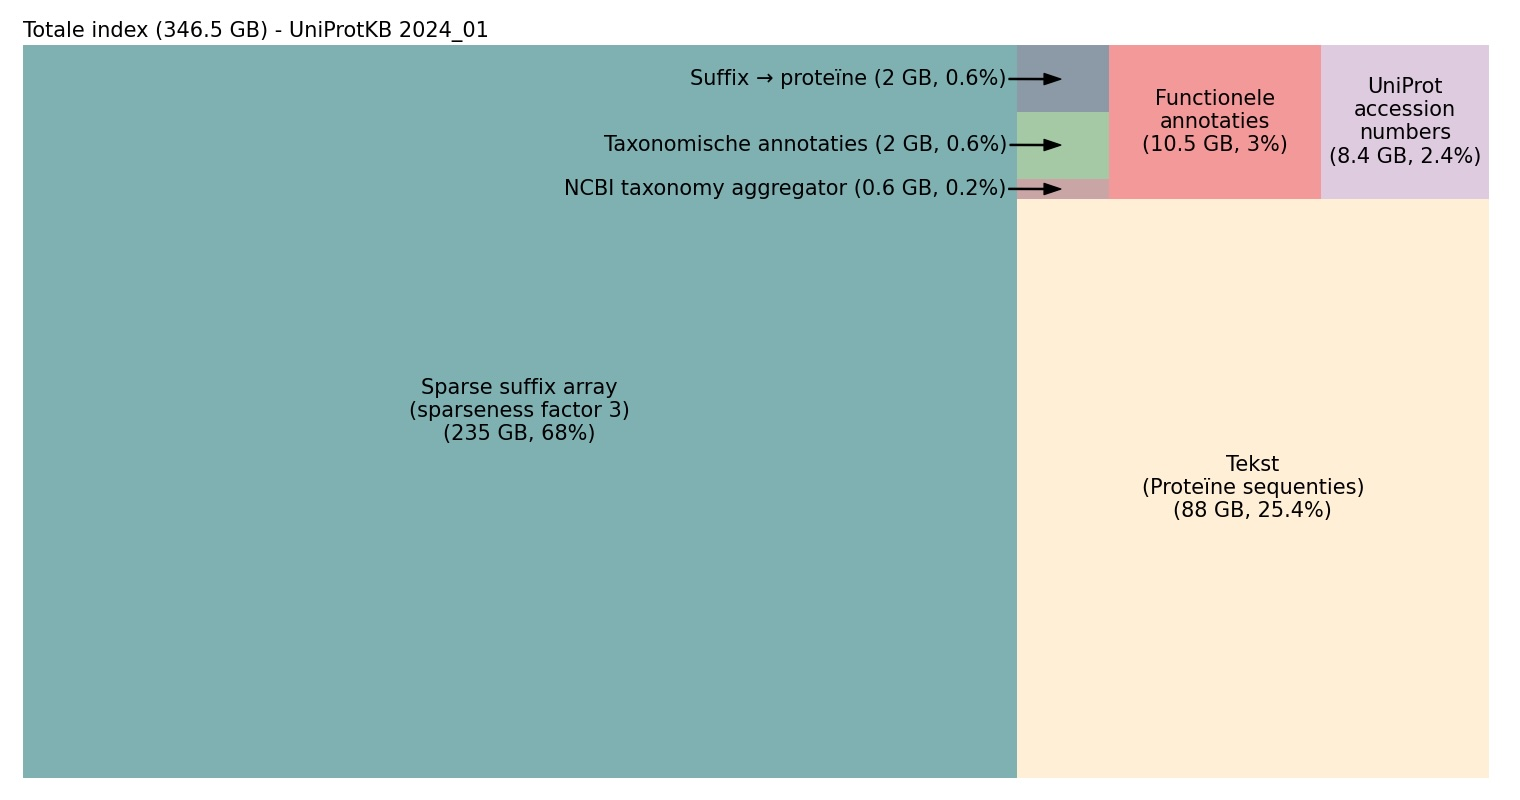
\includegraphics[width=0.76\linewidth]{uniprot_memory_treemap}
    \caption{Visualisatie van het totale geheugenverbruik voor de index gebouwd op basis van UniProtKB 2024\_01, gebruikmakende van sparseness factor $k = 3$ voor de SSA.
    In het totaal vraagt deze index 346.5 GB RAM, waarvan het grootste stuk gebruikt wordt door de SSA en de proteïne sequenties (de tekst) zelf.
    Naast de twee onderdelen die nodig zijn voor het matchen van de suffixen, is er nog een kleine 25 GB extra RAM nodig om de Unipept analyses aan te kunnen bieden, of om de ID's van de gevonden matches terug te kunnen geven.}
    \label{fig:uniprot_memory_treemap}
\end{figure}
\newpage
\section{Aanbieden van de nieuwe indexstructuur}\label{sec:aanbieden-van-de-nieuwe-indexstructuur}
In alle eerder vermelde benchmarks bespraken we enkel de zoektijd van een peptidebestand.
Bij het opstarten moeten we echter \textbf{eerst de indexstructuur inladen in RAM}.
Dit alleen duurt 20 tot 25 minuten.
We willen dit inladen slechts eenmalig doen om dan alle requests onmiddellijk te kunnen afhandelen.
Dit doen we aan de hand van een simpele \textbf{webserver} met de Axum crate~\cite{axum}.
Deze webserver laadt de indexstructuur in bij het opstarten, en blijft daarna wachten op HTTP-requests die een JSON-object bevatten met daarin de peptiden die we willen zoeken.
Op deze manier is dit probleem elegant opgelost, en kunnen we bovendien aan de hand van \textbf{JSON-bestanden} erg makkelijk de input verwerken, en de resultaten terugsturen.
Codefragment~\ref{fig:webserver_json_input} en~\ref{fig:webserver_json_output} geven een voorbeeld input en output.

\begin{listing}[H]
    \begin{minted}[frame=lines,framesep=2mm,linenos]{JSON}
{
  "peptides": [
    "LAKLFISAV",
    "ACCISDJLSDAAC"
  ],
  "equalize_I_and_L": true,
  "cutoff": 10000
}
    \end{minted}
    \caption{Voorbeeld JSON-input voor de webserver waarbij de peptiden \texttt{LAKLFISAV} en \texttt{ACCISDJLSDAAC} gezocht worden.
    Tijdens het zoeken worden I en L gelijkgesteld, en wordt de drempelwaarde B=10\thinspace000 gebruikt.
    Indien er meer matches zijn dan de drempelwaarde B, worden er slechts B matches terug gegeven en de resulterende LCA op 1 gezet.
    Dit laatste argument zou ook weggelaten kunnen worden aangezien de standaardwaarde gebruikt wordt.}
    \label{fig:webserver_json_input}
\end{listing}

\begin{listing}[h!]
    \begin{minted}[frame=lines,framesep=2mm,linenos]{JSON}
{
  "result": [
    {
      "sequence": "LAKLFISAV",
      "lca": 2,
      "taxa": [
        2249812,
        1871048,
        1262816,
        1869212
      ],
      "uniprot_accessions": [
        "A0A365TSP2",
        "A0A7C5MYD2",
        "R6CCR3",
        "A0A7V8W1P5"
      ],
      "fa": {
        "counts": {
          "EC": 0,
          "IPR": 4,
          "GO": 3,
          "all": 4
        },
        "data": {
          "GO:0005886": 2,
          "IPR:IPR025970": 1,
          "IPR:IPR010656": 2,
          "GO:0000271": 1,
          "IPR:IPR007267": 1,
          "IPR:IPR004681": 2,
          "GO:0016020": 1,
          "GO:0022857": 2
        }
      },
      "cutoff_used": false
    }
  ]
}
    \end{minted}
    \caption{Output van de input gebruikt in Codefragment~\ref{fig:webserver_json_input}.
    Hierbij bevat de sleutel \texttt{result} één element voor elke peptide die minstens één match opleverde.
    Peptiden zonder match worden dus simpelweg weggelaten in de output.
    Elk element bevat de berekende LCA voor alle matches, het taxon ID dat overeenkomt met elke match en het UniProt accession number voor elke match.
    Verder bevat de sleutel \texttt{fa} de functionele analyse zoals deze op dit moment door de Unipept API al teruggegeven wordt.
    Tot slot is er ook nog een extra sleutel \texttt{cutoff\_used} die aanduidt als de bovengrens voor maximaal aantal matches gebruikt is.
    In dit geval stond deze bovengrens B op 10\thinspace000 matches.
    Indien deze wel gebruikt is zal de LCA automatisch op 1 gezet worden en zullen er exact B matches teruggegeven worden (en dus ook matches weggelaten worden).}
    \label{fig:webserver_json_output}
\end{listing}

\section{Productiepijplijn}
Om een nieuwe versie van de index voor UniProtKB in productie te brengen zijn verschillende stappen nodig.
Een groot deel hiervan valt buiten het domein van deze masterproef.
Zo moet de nieuwe databank eerst gedownload worden, moet alle data die Unipept hieruit nodig heeft geëxtraheerd worden, om daarna een reeks aan transformaties uit te voeren.
De masterproef van medestudent Stijn De Clercq gaat hier dieper op in, en welke verbetering hieraan toegebracht zijn het afgelopen jaar.
Dankzij zijn werk is het veel gemakkelijker geworden om deze nieuwe index te integreren in de Unipept pijplijn.
De output van deze pijplijn levert een reeks \texttt{tsv}\footnote{Tab-Separated Values} bestanden op, die gebruikt worden als input om de indexstructuur op te bouwen.
Aangezien we de index enkel kunnen bouwen op de HPC vanwege de nodige hoeveelheid RAM, moet dit bestand ook verplaatst worden naar de HPC\@.
Dit gaat vrij snel aangezien alle communicatie binnen het UGent-netwerk gebeurt aan een snelheid van 1 Gbps.
Daarna wordt er een job op de HPC in de wachtrij gezet om de effectieve nieuwe SSA op te bouwen.
Hierbij moet eerst wat tijd gerekend worden waarbij de job in de wachtrij staat.
Meestal duurt dit niet langer dan enkele uren, waarna de berekening zelf een 6-tal uur in beslag neemt.
Eens de HPC klaar is met het bouwen van de index moet de resulterende SSA van ongeveer 235 GB verplaatst worden naar alle Unipept servers die de index zullen hosten.
Opnieuw is dit communicatie binnen het UGent-netwerk, waardoor dit ongeveer een half uur in beslag neemt.
Tot slot moet de index op alle servers opgestart worden.
Zoals vermeld in sectie~\ref{sec:aanbieden-van-de-nieuwe-indexstructuur}, duurt dit ongeveer 20--25 minuten, waarna de index binnenkomende requests kan verwerken.
